\documentclass[../psets.tex]{subfiles}

\pagestyle{main}
\renewcommand{\leftmark}{Problem Set \thesection}
\setcounter{section}{3}
\setenumerate[1]{label={\textbf{\arabic*.}}}
\setenumerate[2]{label={(\arabic*)}}

\begin{document}




\section{Final Explicitly Solvable Cases}
\subsection*{Required Problems}
\begin{enumerate}
    \item \marginnote{11/2:}Use Duhamel's formula to solve the initial value problem
    \begin{equation*}
        y' =
        \begin{pmatrix}
            0 & -1\\
            1 & 0\\
        \end{pmatrix}
        y+
        \begin{pmatrix}
            -t\\
            t\\
        \end{pmatrix}
        ,\quad
        y(0) =
        \begin{pmatrix}
            1\\
            0\\
        \end{pmatrix}
    \end{equation*}
    \begin{proof}
        Diagonalizing $A$ reveals that
        \begin{equation*}
            \underbrace{
                \begin{pmatrix}
                    0 & -1\\
                    1 & 0\\
                \end{pmatrix}
            }_A = \underbrace{
                \begin{pmatrix}
                    i & -i\\
                    1 & 1\\
                \end{pmatrix}
            }_Q\underbrace{
                \begin{pmatrix}
                    i & 0\\
                    0 & -i\\
                \end{pmatrix}
            }_B\underbrace{
                \begin{pmatrix}
                    -i/2 & 1/2\\
                    i/2 & 1/2\\
                \end{pmatrix}
            }_{Q^{-1}}
        \end{equation*}
        Thus,
        \begin{equation*}
            \e[tA] = Q\e[tB]Q^{-1}
            = Q
            \begin{pmatrix}
                \e[it] & 0\\
                0 & \e[-it]\\
            \end{pmatrix}
            Q^{-1}
        \end{equation*}
        We have that
        \begin{align*}
            y(t) ={}& \e[tA]y_0+\int_0^t\e[(t-\tau)A]f(\tau)\dd\tau\\
            \begin{split}
                ={}&
                \begin{pmatrix}
                    i & -i\\
                    1 & 1\\
                \end{pmatrix}
                \begin{pmatrix}
                    \e[it] & 0\\
                    0 & \e[-it]\\
                \end{pmatrix}
                \begin{pmatrix}
                    -i/2 & 1/2\\
                    i/2 & 1/2\\
                \end{pmatrix}
                \begin{pmatrix}
                    1\\
                    0\\
                \end{pmatrix}\\
                &+\int_0^t
                \begin{pmatrix}
                    i & -i\\
                    1 & 1\\
                \end{pmatrix}
                \begin{pmatrix}
                    \e[i(t-\tau)] & 0\\
                    0 & \e[-i(t-\tau)]\\
                \end{pmatrix}
                \begin{pmatrix}
                    -i/2 & 1/2\\
                    i/2 & 1/2\\
                \end{pmatrix}
                \begin{pmatrix}
                    -\tau\\
                    \tau\\
                \end{pmatrix}
                \dd\tau
            \end{split}\\
            ={}&
            \begin{pmatrix}
                \frac{\e[it]+\e[-it]}{2}\\
                \frac{\e[it]-\e[-it]}{2i}\\
            \end{pmatrix}
            +\int_0^t
            \begin{pmatrix}
                \tau\left( \frac{\e[i(t-\tau)]-\e[-i(t-\tau)]}{2i}-\frac{\e[i(t-\tau)]+\e[-i(t-\tau)]}{2} \right)\\
                \tau\left( \frac{\e[i(t-\tau)]-\e[-i(t-\tau)]}{2i}-\frac{\e[i(t-\tau)]+\e[-i(t-\tau)]}{2} \right)\\
            \end{pmatrix}
        \end{align*}
        Substitute sines and cosines and evaluate.
    \end{proof}
    \item Let $A$ be an $n\times n$ complex constant matrix and let $f(t)=\e[\zeta t]p(t)$, where $p(t)$ is a $\C^n$-valued function whose entries are all polynomials. We define $\deg p(t)$ to be the largest of the degrees of its entries. Use Duhamel's formula to prove the following proposition:\par
    If $\zeta$ is not an eigenvalue of $A$, then the solution of $y'=Ay+p(t)\e[\zeta t]$ takes the form
    \begin{equation*}
        \e[tA]z_0+q(t)\e[\zeta t]
    \end{equation*}
    where $z_0$ is a constant vector (\emph{not} necessarily the initial value) and $q(t)$ is a polynomial vector with degree being the same as $p(t)$. If $\zeta$ is an eigenvalue of $A$ with algebraic multiplicity $\alpha$, then the solution of $y'=Ay+\e[\zeta t]p(t)$ takes the form
    \begin{equation*}
        \e[tA]z_0+r(t)\e[\zeta t]
    \end{equation*}
    where $z_0$ is a constant vector (\emph{not} necessarily the initial value) and $r(t)$ is a polynomial vector with degree $\deg p(t)+\alpha$.
    \begin{proof}
        Shao said in office hours that this question cannot be answered, and as such he would cancel it; he copied it out of Teschl but it had an error as written.
    \end{proof}
    \item We know that for the driven harmonic oscillator equation
    \begin{equation*}
        x''+\omega_0^2x = H_0\cos\omega t
    \end{equation*}
    when $\omega=\omega_0$, the solution grows unboundedly. However, what if $\omega\neq\omega_0$ but is very close?\par
    For simplicity, suppose that $H_0>0$ and the initial values $x(0),x'(0)$ are real numbers that are very small compared to $H_0/|\omega^2-\omega_0^2|$, say,
    \begin{equation*}
        |x(0)|+|x'(0)| < \frac{\varepsilon H_0}{|\omega^2-\omega_0^2|}
    \end{equation*}
    Suppose also that $|\omega-\omega_0|$ is very small compared to $\omega_0$, say
    \begin{equation*}
        |\omega-\omega_0| < \varepsilon\omega_0
    \end{equation*}
    Lastly, suppose that the initial values are small compared to the eigenfrequency, say
    \begin{equation*}
        |x(0)|+|x'(0)| < \varepsilon\omega_0
    \end{equation*}
    Prove that there is a sequence of times $t_k\to +\infty$ such that
    \begin{equation*}
        x(t_k) > 2(1-\varepsilon)\cdot\frac{H_0}{|\omega^2-\omega_0^2|}
        \approx \frac{1}{\varepsilon}
    \end{equation*}
    That is, the mass point will constantly visit positions very far away from the equilibrium.\par
    \emph{Hint}. Write down the solution first, and then you need to discuss two cases separately: $\omega/\omega_0$ is rational/irrational. In the latter case, you should use the following theorem of Kronecker.
    \begin{theorem}
        Let $\alpha,\beta$ be positive real numbers such that $\alpha/\beta$ is irrational. Then the set $\{(\langle n\alpha\rangle,\langle n\beta\rangle)\mid n\in\N\}$ is dense in the unit sphere $[0,1]\times[0,1]$, where $\langle\cdot\rangle$ denotes the decimal part of a real number.
    \end{theorem}
    \begin{proof}
        % Using the substitutions
        % \begin{align*}
        %     \sin\theta &= \frac{\e[i\theta]-\e[-i\theta]}{2i}&
        %     \cos\theta &= \frac{\e[i\theta]+\e[-i\theta]}{2}
        % \end{align*}
        % we may evaluate the integral as follows.
        % \begin{align*}
        %     \text{Int} &= \int_0^t\frac{\sin\omega_0(t-\tau)}{\omega_0}(H_0\cos\omega\tau)\dd\tau\\
        %     &= \frac{H_0}{\omega_0}\int_0^t\frac{\e[i\omega_0(t-\tau)]-\e[-i\omega_0(t-\tau)]}{2i}\cdot\frac{\e[i\omega\tau]+\e[-i\omega\tau]}{2}\dd\tau\\
        %     &= \frac{H_0}{4i\omega_0}\int_0^t\left[ \e[i(\omega_0t-\omega_0\tau+\omega\tau)]+\e[i(\omega_0t-\omega_0\tau-\omega\tau)]-\e[i(\omega\tau-\omega_0t+\omega_0\tau)]-\e[i(\omega_0\tau-\omega_0t-\omega\tau)] \right]\dd\tau\\
        %     &= \frac{H_0}{4i\omega_0}\int_0^t\left[ \e[i(\omega_0t+(\omega-\omega_0)\tau)]+\e[i(\omega_0t-(\omega_0+\omega)\tau)]-\e[i((\omega+\omega_0)\tau-\omega_0t)]-\e[i((\omega_0-\omega)\tau-\omega_0t)] \right]\dd\tau\\
        % \end{align*}


        From HW3, the given driven harmonic oscillator equation is solved by
        \begin{align*}
            x(t) &= x(0)\cos\omega_0t+x'(0)\frac{\sin\omega_0t}{\omega_0}+\int_0^t\frac{\sin\omega_0(t-\tau)}{\omega_0}(H_0\cos\omega\tau)\dd\tau\\
            &= x(0)\cos\omega_0t+x'(0)\frac{\sin\omega_0t}{\omega_0}+\frac{H_0}{\omega^2-\omega_0^2}(\cos\omega_0t-\cos\omega t)
        \end{align*}
        We have that $|x(0)\cos\omega_0t|\leq|x(0)|$ and $|x'(0)\sin\omega_0t|\leq|x'(0)|$ and $|x'(0)|<\varepsilon\omega_0$ and $|x(0)|<\varepsilon H_0/|\omega^2-\omega_0^2|$. Thus
        \begin{align*}
            \left| x(0)\cos\omega_0t+x'(0)\frac{\sin\omega_0t}{\omega_0} \right| &\leq |x(0)\cos\omega_0t|+\frac{1}{\omega_0}|x'(0)\sin\omega_0t|\\
            &\leq |x(0)|+\frac{|x'(0)|}{\omega_0}\\
            &< |x(0)|+\varepsilon\\
            &< \frac{\varepsilon H_0}{|\omega^2-\omega_0^2|}+\varepsilon\\
            &= \varepsilon\left( \frac{H_0}{|\omega^2-\omega_0^2|}+1 \right)
        \end{align*}
        We also have that
        \begin{align*}
            \left| \frac{H_0}{\omega^2-\omega_0^2}(\cos\omega_0t-\cos\omega t) \right| &= \frac{H_0}{|\omega^2-\omega_0^2|}\cdot|\cos\omega_0t-\cos\omega t|\\
            &\leq \frac{H_0}{|\omega^2-\omega_0^2|}\cdot 2
        \end{align*}
        It follows that
        \begin{align*}
            |x(t)| &< \frac{2H_0}{|\omega^2-\omega_0^2|}+\frac{\varepsilon H_0}{|\omega^2-\omega_0^2|}+\varepsilon\\
            &= (2+\varepsilon)\cdot\frac{H_0}{|\omega^2-\omega_0^2|}+\varepsilon
        \end{align*}
    \end{proof}
    \item Sketch the phase diagram of the following linear autonomous systems. Also clearly indicate
    \begin{itemize}
        \item The eigenvalues and eigenvectors;
        \item The stable and unstable subspaces (if the eigenvalues are not purely imaginary);
        \item The shape and direction of the trajectories (attracted/repelled by the fixed point).
    \end{itemize}
    \begin{enumerate}
        \item 
        \begin{equation*}
            y' =
            \begin{pNiceMatrix}
                \frac{1}{2} & 1\\
                -1 & \frac{1}{2}\\
            \end{pNiceMatrix}
            y
        \end{equation*}
        \begin{proof}
            Using techniques from previous weeks, we can diagonalize $A$ as follows.
            \begin{equation*}
                \begin{pNiceMatrix}
                    \frac{1}{2} & 1\\
                    -1 & \frac{1}{2}\\
                \end{pNiceMatrix}
                =
                \begin{pmatrix}
                    -i & i\\
                    1 & 1\\
                \end{pmatrix}
                \begin{pNiceMatrix}
                    \frac{1}{2}+i & 0\\
                    0 & \frac{1}{2}-i\\
                \end{pNiceMatrix}
                \begin{pNiceMatrix}
                    \frac{i}{2} & \frac{1}{2}\\
                    -\frac{i}{2} & \frac{1}{2}\\
                \end{pNiceMatrix}
            \end{equation*}
            Thus, the eigenvalues and corresponding eigenvectors of $A$ are
            \begin{empheq}[box=\fbox]{align*}
                \lambda &= \frac{1}{2}+i&
                    \bar{\lambda} &= \frac{1}{2}-i&
                v &=
                \begin{pmatrix}
                    -i\\
                    1\\
                \end{pmatrix}&
                    \bar{v} &=
                    \begin{pmatrix}
                        i\\
                        1\\
                    \end{pmatrix}
            \end{empheq}
            It follows that
            \begin{empheq}[box=\fbox]{align*}
                \text{stable subspace} &= \{0\}&
                \text{unstable subspace} &= \R^2
            \end{empheq}
            Moreover, the shape and direction of the trajectories (using the convention from Q5(2)) are
            \begin{equation*}
                \boxed{\text{Spiral source; repelled}}
            \end{equation*}
            Therefore,
            \begin{center}
                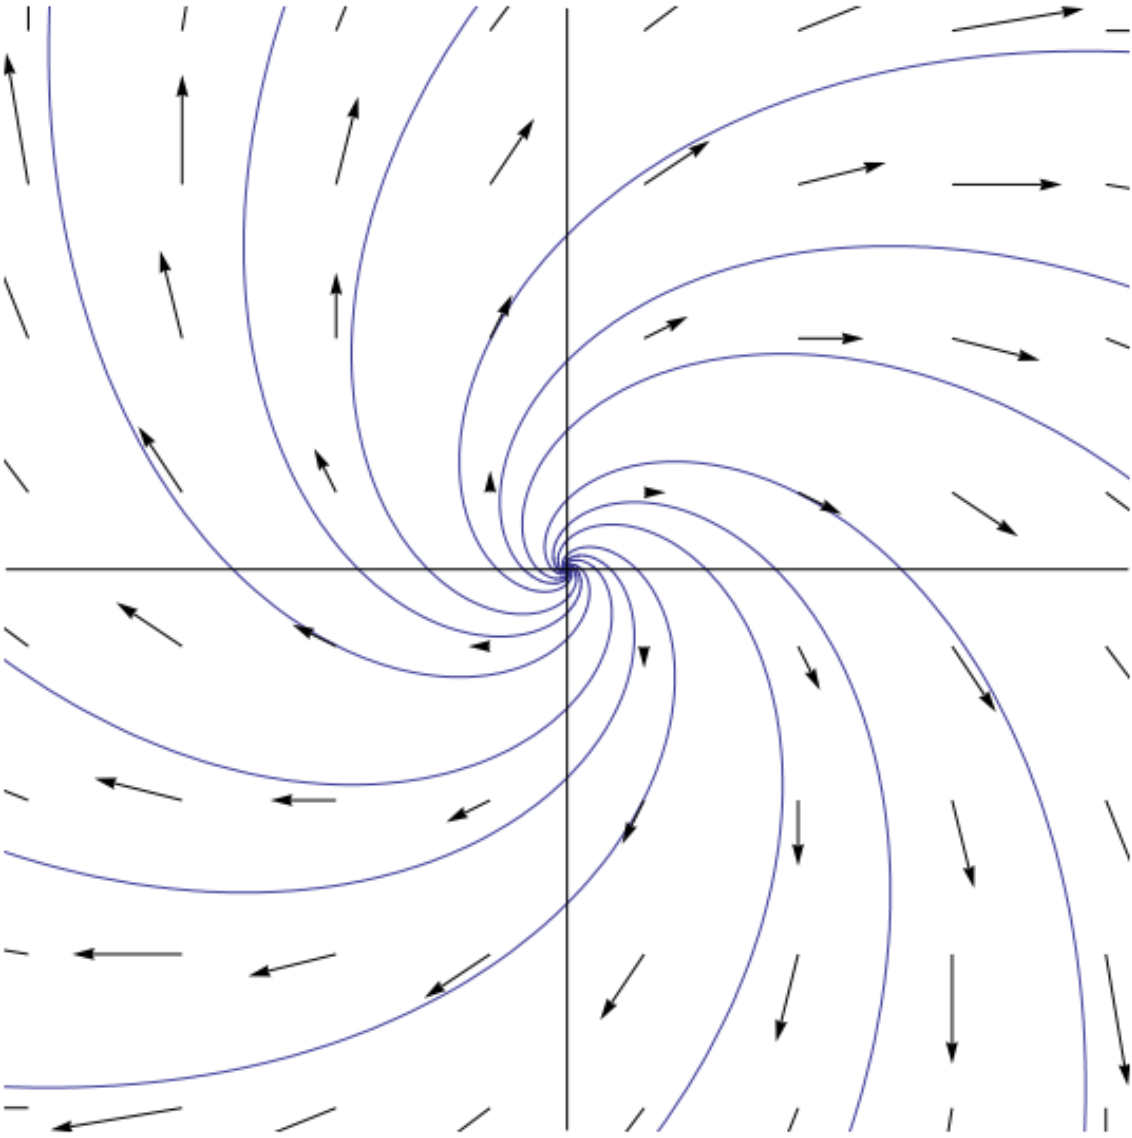
\includegraphics[width=0.256\linewidth]{../ExtFiles/planarComplexa.png}
            \end{center}
        \end{proof}
        \item 
        \begin{equation*}
            y' =
            \begin{pmatrix}
                1 & 2\\
                -2 & 1\\
            \end{pmatrix}
            y
        \end{equation*}
        \begin{proof}
            This question is entirely analogous to part (1). Indeed, we get eigenvalues and eigenvectors
            \begin{empheq}[box=\fbox]{align*}
                \lambda &= 1+2i&
                    \bar{\lambda} &= 1-2i&
                v &=
                \begin{pmatrix}
                    -i\\
                    1\\
                \end{pmatrix}&
                    \bar{v} &=
                    \begin{pmatrix}
                        i\\
                        1\\
                    \end{pmatrix}
            \end{empheq}
            subspaces
            \begin{empheq}[box=\fbox]{align*}
                \text{stable subspace} &= \{0\}&
                \text{unstable subspace} &= \R^2
            \end{empheq}
            and shape and direction
            \begin{equation*}
                \boxed{\text{Spiral source; repelled}}
            \end{equation*}
            Therefore,
            \begin{center}
                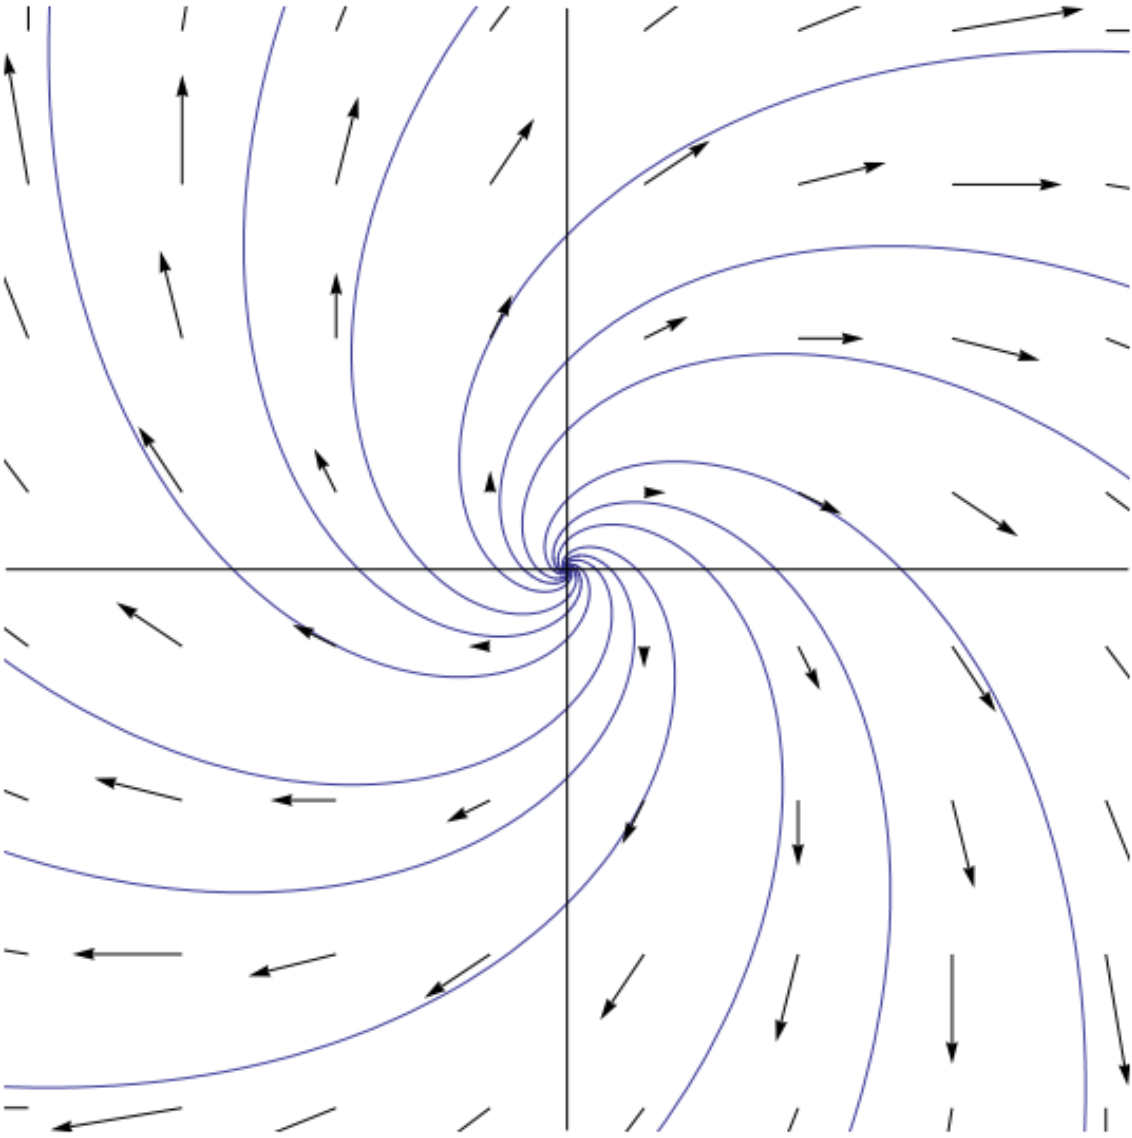
\includegraphics[width=0.256\linewidth]{../ExtFiles/planarComplexa.png}
            \end{center}
        \end{proof}
        \item 
        \begin{equation*}
            y' =
            \begin{pNiceMatrix}
                1 & \frac{1}{2}\\
                \frac{1}{2} & 1\\
            \end{pNiceMatrix}
            y
        \end{equation*}
        \begin{proof}
            This time our diagonalization gives real, distinct eigenvalues and eigenvectors
            \begin{empheq}[box=\fbox]{align*}
                \lambda_1 &= \frac{3}{2}&
                    \lambda_2 &= \frac{1}{2}&
                v_1 &=
                \begin{pmatrix}
                    1\\
                    1\\
                \end{pmatrix}&
                    v_2 &=
                    \begin{pmatrix}
                        -1\\
                        1\\
                    \end{pmatrix}
            \end{empheq}
            Since both eigenvalues are greater than zero, we have subspaces
            \begin{empheq}[box=\fbox]{align*}
                \text{stable subspace} &= \{0\}&
                \text{unstable subspace} &= \R^2
            \end{empheq}
            Since we have two positive real eigenvalues, we have shape and direction
            \begin{equation*}
                \boxed{\text{Source; repelled}}
            \end{equation*}
            Additionally, the phase diagram will have many curves of the form $v_2=v_1^{\lambda_2/\lambda_1}$, i.e., $v_2=v_1^{1/3}$, or $v_1=v_2^3$.
            \begin{center}
                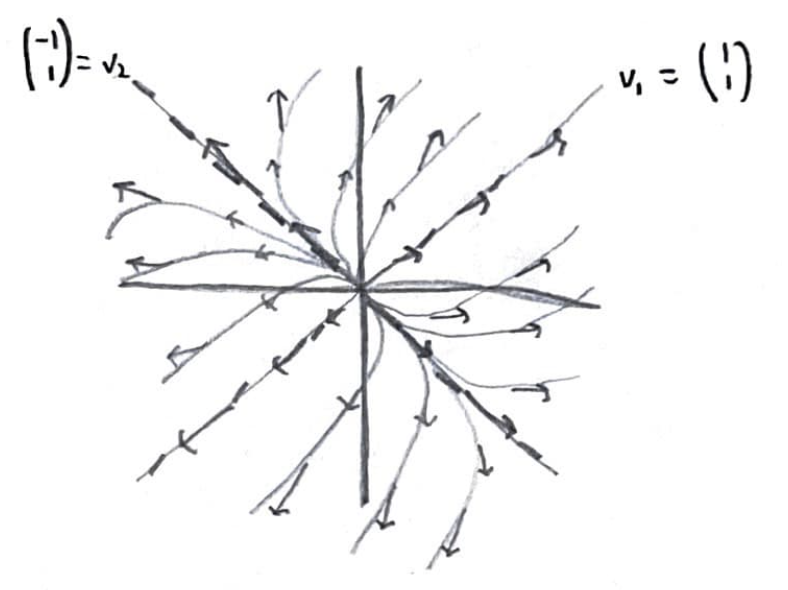
\includegraphics[width=0.4\linewidth]{../ExtFiles/pset4_4-3.png}
            \end{center}
        \end{proof}
        \item 
        \begin{equation*}
            y' =
            \begin{pmatrix}
                -1 & 1\\
                0 & 1\\
            \end{pmatrix}
            y
        \end{equation*}
        \begin{proof}
            Once again, we get real distinct eigenvalues and eigenvectors, but this time our eigenvalues have opposite signs.
            \begin{empheq}[box=\fbox]{align*}
                \lambda_1 &= 1&
                    \lambda_2 &= -1&
                v_1 &=
                \begin{pmatrix}
                    1\\
                    2\\
                \end{pmatrix}&
                    v_2 &=
                    \begin{pmatrix}
                        1\\
                        0\\
                    \end{pmatrix}
            \end{empheq}
            Because of their opposite signs, we have our first nontrivial stable subspace (corresponding to the negative eigenvalue).
            \begin{empheq}[box=\fbox]{align*}
                \text{stable subspace} &= \spn\{v_2\}&
                \text{unstable subspace} &= \spn\{v_1\}
            \end{empheq}
            Likewise, it follows that
            \begin{equation*}
                \boxed{\text{Saddle; both (depends on the subspace)}}
            \end{equation*}
            Additionally, we will have a power function of a negative power $v_2=v_1^{\lambda_2/\lambda_1}$, i.e., $v_2=1/v_1$.
            \begin{center}
                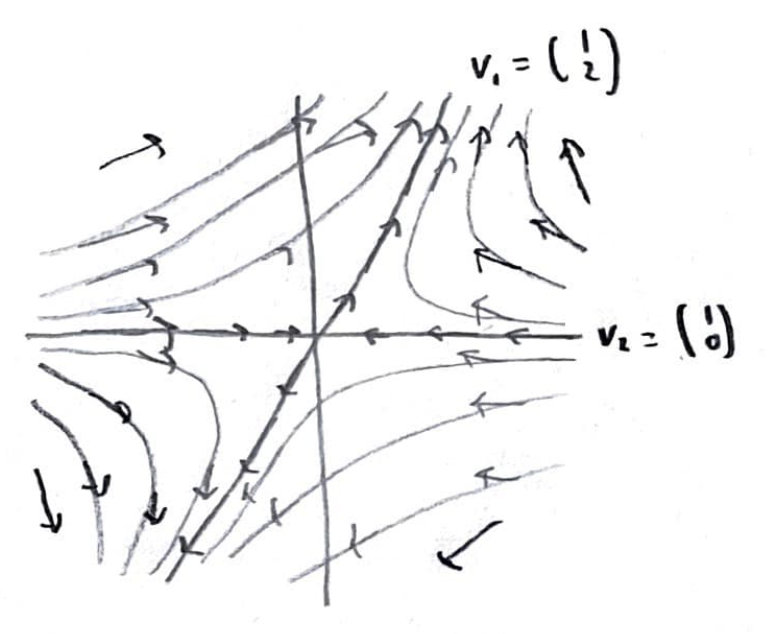
\includegraphics[width=0.4\linewidth]{../ExtFiles/pset4_4-4.png}
            \end{center}
        \end{proof}
        \item 
        \begin{equation*}
            y' =
            \begin{pmatrix}
                2 & 1\\
                0 & 2\\
            \end{pmatrix}
            y
        \end{equation*}
        \begin{proof}
            This matrix is already in JNF with a single Jordan block. Thus, we have one lone eigenvalue $\lambda$, an eigenvector $v$, and a generalized eigenvector $u$ as follows.
            \begin{empheq}[box=\fbox]{align*}
                \lambda &= 2&
                v &=
                \begin{pmatrix}
                    1\\
                    0\\
                \end{pmatrix}&
                    u &=
                    \begin{pmatrix}
                        0\\
                        1\\
                    \end{pmatrix}
            \end{empheq}
            Evidently, $\lambda>0$, so
            \begin{empheq}[box=\fbox]{align*}
                \text{stable subspace} &= \{0\}&
                \text{unstable subspace} &= \R^2
            \end{empheq}
            Now there is not a specific naming convention for the this shape in Q5(2), so we will call it "distorted source:"
            \begin{equation*}
                \boxed{\text{Distorted source; repelled}}
            \end{equation*}
            Additionally, we will have a function of the form $v=u+u\ln u$.
            \begin{center}
                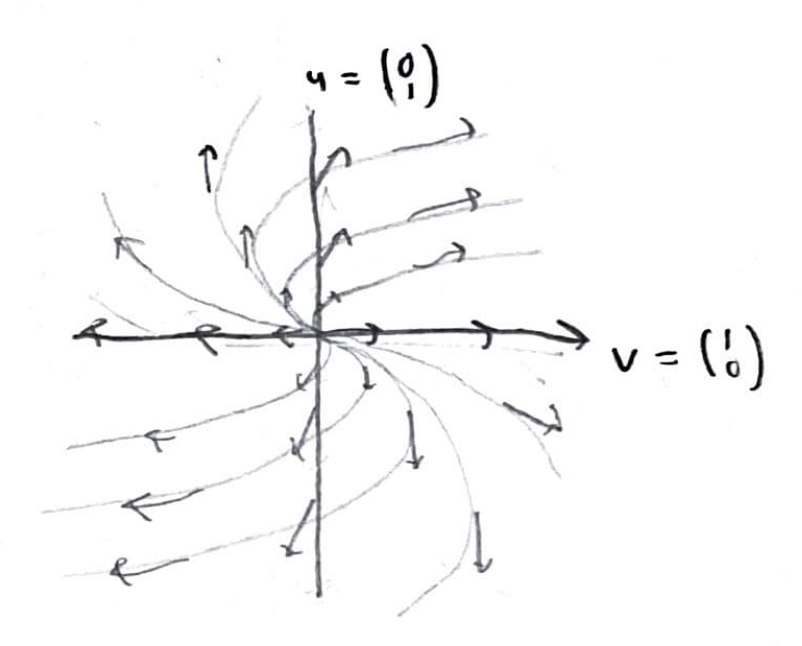
\includegraphics[width=0.4\linewidth]{../ExtFiles/pset4_4-5.png}
            \end{center}
        \end{proof}
    \end{enumerate}
    \item Given a matrix
    \begin{equation*}
        A =
        \begin{pmatrix}
            a & b\\
            c & d\\
        \end{pmatrix}
    \end{equation*}
    the number $a+d$ is called the trace of $A$ and is denoted by $\Trc A$.
    \begin{enumerate}
        \item Prove that $\Trc A$ is invariant under similarity, and show that
        \begin{align*}
            \chi_A(z) &= z^2-(\Trc A)z+\det A&
            \det\e[A] &= \e[\Trc A]
        \end{align*}
        \begin{proof}
            \underline{Left equality above}: We have that
            \begin{align*}
                \chi_A(z) &= \det(A-zI)\\
                &= \det
                \begin{pmatrix}
                    a-z & b\\
                    c & d-z\\
                \end{pmatrix}\\
                &= (a-z)(d-z)-bc\\
                &= z^2-az-dz+ad-bc\\
                &= z^2-(\underbrace{a+d}_{\Trc A})z+(\underbrace{ad-bc}_{\det A})
            \end{align*}
            as desired.\par
            \underline{Invariance of the trace under similarity}: Suppose $A\sim B$. Then since similar matrices have the same characteristic polynomial, we have by the left equality above that
            \begin{align*}
                \chi_A(z) &= \chi_B(z)\\
                z^2-(\Trc A)z+\det A &= z^2-(\Trc B)z+\det B\\
                \Trc A &= \Trc B
            \end{align*}
            as desired.\par
            \underline{Right equality above}: Suppose $\e[A]=Q\e[B]Q^{-1}$ where $B$ is in JNF. Then
            \begin{align*}
                \det\e[A] &= \det\e[B]\\
                &= \e[\lambda_1]\cdot\e[\lambda_2]\\
                &= \e[\lambda_1+\lambda_2]\\
                &= \e[\Trc B]\\
                &= \e[\Trc A]
            \end{align*}
            where we have the first equality because the determinant is invariant under similarity; the second equality because $\e[B]$ is upper triangular, the determinant of an upper triangular matrix is equal to the product of the diagonal entries, and the diagonal entries of $\e[B]$ are the exponentials of the eigenvalues of $A$; and the remainder of the equalities for fairly evident reasons.
        \end{proof}
        \item Suppose $A$ is a real matrix. We have discussed the phase diagram of the linear autonomous system $y'=Ay$ and classified them into several cases according to the eigenvalues of $A$: Spiral source/sink (complex eigenvalues with positive/negative real part), ellipse (purely imaginary eigenvalues), saddle (real eigenvalue with opposite sign), source/sink (positive/negative real eigenvalue). Now the eigenvalues are completely determined by the tuple of real numbers $(T,D)=(\Trc A,\det A)$. Split the $(T,D)$ plane into several parts in which the various cases discussed this Monday occur.
        \begin{proof}
            We have that
            \begin{center}
                \footnotesize
                \begin{tikzpicture}[scale=0.5]
                    \fill [ret] (0,0) parabola (4,4) -- (4,0);
                    \fill [ret!20!ort] (0,0) parabola (4,4) -- (0,4);
                    \fill [ylt!20!ort] (0,0) parabola (-4,4) -- (0,4);
                    \fill [ylt] (0,0) parabola (-4,4) -- (-4,0);
                    \fill [puz] (-4,-4) rectangle (4,0);
            
                    \draw
                        (-4,0) -- (4,0) node[right]{$T$}
                        (0,-4) -- (0,4) node[above]{$D$}
                    ;
            
                    \draw [rex,ultra thick] (0,0) parabola (4,4);
                    \draw [ylx,ultra thick] (0,0) parabola (-4,4);
                    \draw [orx,ultra thick] (0,0) -- (0,4);
            
                    \filldraw [fill=white,thick] circle (1.5mm);
                \end{tikzpicture}
            \end{center}
            We will identify the various colored regions in lines throughout the following derivation. Let's begin.\par
            Suppose we have two identical eigenvalues $a$. Then the shape will be distorted source if $a>0$ and distorted sink if $a<0$. In this case $T=2a$ and $D=a^2$. It follows by solving the first equation for $a$ and substituting it into the second that
            \begin{equation*}
                D = \frac{1}{4}T^2
            \end{equation*}
            Thus, every $(T,D)$ falling along this positive portion of this parabola (the red parabola in the diagram) corresponds to a distorted source, and vice versa for the negative portion (yellow).\par
            Suppose $\lambda_1=a+bi$ and $\lambda_2=a-bi$. Then $T=2a$ and $D=a^2+b^2$. Substituting as before, we obtain
            \begin{equation*}
                D = \frac{1}{4}T^2+b^2
            \end{equation*}
            where $b^2>0$. Thus, every $(T,D)$ lying \emph{above} the parabola corresponds to a spiral. For positive $T$ (the red/orange shaded region), we have a spiral source, and vice versa for negative $T$.\par
            Suppose $\lambda_1=bi$ and $\lambda_2=-bi$. Then $T=0$ and $D=b^2$. Thus, the orange part of the vertical axis corresponds to all ellipses.\par
            Now suppose $\lambda_1,\lambda_2\in\R$. WLOG let $\lambda_2>\lambda_1$. Define $\delta:=\lambda_2-\lambda_1$. Then $T=2\lambda_1+\delta$ and $D=\lambda_1^2+\delta\lambda_1$. Substituting as before, we obtain
            \begin{equation*}
                D = \left( \frac{T-\delta}{2} \right)^2+\delta\cdot\frac{T-\delta}{2}
                = \frac{1}{4}T^2-\frac{\delta^2}{4}
            \end{equation*}
            If $D>0$, then
            \begin{align*}
                0 &< \frac{1}{4}T^2-\frac{\delta^2}{4}\\
                \delta &< T\\
                \lambda_2-\lambda_1 &< \lambda_1+\lambda_2\\
                0 &< 2\lambda_1\\
                0 &< \lambda_1 < \lambda_2
            \end{align*}
            Thus, the red shaded region lying above the $T$ axis but below the red half-parabola corresponds to all sources. Assuming $D<0$ leads in an analogous fashion to the conclusion that $0>\lambda_2>\lambda_1$, meaning that the yellow shaded region lying above the $T$ axis but below the yellow half-parabola corresponds to all sinks.\par
            Lastly, any point lying below the $T$ axis must have one positive and one negative eigenvalue: $D=\lambda_1\lambda_2<0$ implies either $\lambda_1<0$ or $\lambda_2<0$ but not both. Thus, the purple shaded region corresponds to saddles.\par
            As a final comment, note that there are several other types of graphs that we did not talk about on Monday that also have their place on this diagram, e.g., the origin corresponds to uniform motion.
        \end{proof}
    \end{enumerate}
\end{enumerate}


\subsection*{Bonus Problem}
In this problem, we aim to explore more physical applications of the harmonic oscillator equation to the study of linear wave equations.
\begin{enumerate}
    \item Suppose we have a perfect string undergoing vertical vibrations of small amplitude within a given vertical plane. The following physical quantities are relevant.
    \begin{center}
        \begin{tikzpicture}[scale=1.5]
            \footnotesize
            \draw (-0.5,0) -- (2,0);
            \draw (0,0) node[below]{$x$} -- node[right]{$u(x,t)$} ++(0,1.5) coordinate (b1)
                -- node[below]{$\Delta x$} ++(1.5,0) coordinate (a1)
                -- node[right]{$\Delta u$} ++(0,1) coordinate (b2)
                -- ++(1,0) coordinate (a2)
            ;
    
            \draw [-latex] (b2) -- ++(1,0.5) coordinate (c2) node[right]{$T(x+\Delta x,t)$};
            \pic [draw,angle radius=0.6cm,angle eccentricity=1.1,pic text={$\theta(x+\Delta x,t)$},pic text options={right,yshift=1pt}] {angle=a2--b2--c2};
    
            \draw [-latex] (b1) -- ++(-130:1cm) node[left]{$T(x,t)$};
            \path (b1) -- ++(45:1cm) coordinate (c1);
            \pic [draw,angle radius=0.6cm,angle eccentricity=1,pic text={$\theta(x,t)$},pic text options={right,yshift=1pt}] {angle=a1--b1--c1};
    
            \draw [ultra thick] (b1) to[out=50,in=-150,looseness=0.7] (b2);
        \end{tikzpicture}
    \end{center}
    \begin{itemize}
        \item $u(x,t)$: Vertical displacement of the string from the $x$ axis at position $x$ and time $t$.
        \item $\theta(x,t)$: The angle between the string and a horizontal line at position $x$ and time $t$.
        \item $T(x,t)\equiv T_0$: The tension in the string, which is assumed to be constant for a perfect string.
        \item $\rho_0$: The mass density of the string, which is assumed to be constant for a perfect string.
        \item $f(x,t)$: The external force exerted on the strong at position $x$ and time $t$.
    \end{itemize}
    Analyze the forces exerted on the small portion of the string highlighted in bold to derive the following partial differential equation.
    \begin{equation*}
        \rho_0\sqrt{1+\left( \pdv{u}{x} \right)^2}\pdv[2]{u}{t} = T_0\cos\theta\pdv{\theta}{x}+f(x,t)
    \end{equation*}
    When the displacement is small, conclude that this differential equation reduces to the linear wave equation
    \begin{equation*}
        \pdv[2]{u}{t}-c^2\pdv[2]{u}{x} = \frac{f(x,t)}{\rho_0}
    \end{equation*}
    where $c=\sqrt{T_0/\rho_0}$ has units of speed. \emph{Hint}: When the displacement is small, $\pdv*{u}{x}$ is small, and $\theta\approx\tan\theta\approx\pdv*{u}{x}$.\par
    If the string is undergoing unconstrained vibration, that is, there is no boundary condition and the string extends to infinity, then with a linear change of variable $\xi=x+ct$, $\eta=x-ct$, and $w(\xi,\eta)=u(x,t)$, the linear wave equation becomes
    \begin{equation*}
        \pdv{w}{\xi}{\eta} = \frac{f(x,t)}{\rho_0}
    \end{equation*}
    Integrating twice, one can obtain the following theorem.
    \begin{theorem}[d'Alembert]
        The initial value problem for the linear wave equation
        \begin{gather*}
            \pdv[2]{u}{t}-c^2\pdv[2]{u}{x} = \frac{f(x,t)}{\rho_0}\\
            u(x,0) = g(x)
                ,\quad
                {\pdv{u}{t}}(x,0) = h(x)
        \end{gather*}
        without boundary condition at infinity is uniquely solved by
        \begin{equation*}
            u(x,t) = \frac{1}{2}[g(x+ct)+g(x-ct)]+\frac{1}{2c}\int_{x-ct}^{x+ct}h(s)\dd{s}+\frac{1}{2c\rho_0}\int_0^t\int_{x-c(t-\tau)}^{x+c(t-\tau)}f(y,\tau)\dd{y}\dd\tau
        \end{equation*}
    \end{theorem}
    Thus, the vibration of the string without boundary conditions at infinity is uniquely determined by its initial displacement and velocity. The first two terms in d'Alembert's formula can be considered as traveling waves moving at speed $c$, so the parameter $c$ is in fact the speed of transmission.
    \item However, we are now more interested in vibration with constraints. We consider the homogeneous problem (without external force) first.
    \begin{gather*}
        \pdv[2]{u}{t}-c^2\pdv[2]{u}{x} = 0\\
        u(0,t) = u(l,t) \equiv 0
            ,\quad
            {\pdv{u}{t}}(0,t) = {\pdv{u}{t}}(l,t) \equiv 0
    \end{gather*}
    That is, the string is fixed at the endpoints $x=0,l$. Note that the initial conditions (initial displacement and velocity) are not given yet. Determine all particular solutions of the form $u(x,t)=X(x)T(t)$, and explain why such a solution can be understood as a standing wave. Such a solution is called a \textbf{harmonic}. \emph{Hint}: To satisfy the wave equation, there must hold
    \begin{equation*}
        c^2\frac{X''(x)}{X(x)} = \frac{T''(t)}{T(t)}
    \end{equation*}
    Can $X''/X$ and $T''/T$ both equal something other than a constant? How should they match with the boundary condition?
    \item Admit the following fact in the study of Fourier series.\par
    \begingroup
    \itshape
    Any function $u(x)$ on the closed interval $[0,l]$ that has continuous derivatives vanishing at the endpoints up to order 3 can be uniquely represented as a convergent Fourier series
    \begin{equation*}
        u(x) = \sum_{n=1}^\infty c_n\sin\frac{n\pi x}{l}
    \end{equation*}
    where the Fourier coefficients
    \begin{equation*}
        c_n = \frac{2}{l}\int_0^lu(x)\sin\frac{n\pi x}{l}\dd{x}
    \end{equation*}
    The Fourier series can be differentiated twice termwise and still give rise to a convergent Fourier series.
    \endgroup\par
    Use this to solve the following initial-boundary value problem in terms of Fourier series.
    \begin{gather*}
        \pdv[2]{u}{t}-c^2\pdv[2]{u}{x} = 0\\
        u(x,0) = g(x)
            ,\quad
            {\pdv{u}{t}}(x,0) = h(x)
            ,\quad
            u(0,t) = u(l,t) \equiv 0
            ,\quad
            {\pdv{u}{t}}(0,t) = {\pdv{u}{t}}(l,t) \equiv 0
    \end{gather*}
    Assume enough regularity of the known functions, and the Fourier coefficients of $g(x)$ and $h(x)$ are known as $g_n$ and $h_n$, respectively.
    \item Now suppose that there is an external force exerted periodically on the string.
    \begin{equation*}
        f(x,t) = \cos\omega t\sum_{n=1}^\infty f_n\sin\frac{n\pi x}{l}
    \end{equation*}
    Solve the initial-boundary value problem in terms of Fourier series.
    \begin{gather*}
        \pdv[2]{u}{t}-c^2\pdv[2]{u}{x} = \frac{f(x,t)}{\rho_0}\\
        u(x,0) = g(x)
            ,\quad
            {\pdv{u}{t}}(x,0) = h(x)
            ,\quad
            u(0,t) = u(l,t) \equiv 0
            ,\quad
            {\pdv{u}{t}}(0,t) = {\pdv{u}{t}}(l,t) \equiv 0
    \end{gather*}
    Assume enough regularity of the known functions, and the Fourier coefficients of $g(x)$ and $h(x)$ are known as $g_n$ and $h_n$, respectively.\par
    From your expression of the solution, determine which frequencies $\omega$ of the external force $f(x,t)$ give rise to resonance. Explain why the string can play the role of a tuning fork to detect certain frequencies of vibration.
\end{enumerate}




\end{document}